% 2961w - 30p

\documentclass[12pt,letterpaper]{article}
\usepackage{natbib}
\usepackage{pdflscape}
\usepackage{fullpage}
\usepackage{url}
\usepackage{epsfig}
\usepackage{caption}
\usepackage{hyperref}
\usepackage{enumerate}
\usepackage{dcolumn}
\usepackage{lineno}
\usepackage[T1]{fontenc}
\usepackage{textcomp}
\usepackage{float}
\usepackage[osf]{mathpazo}
\usepackage{listings}
\usepackage{color}

\definecolor{dkgreen}{rgb}{0,0.6,0}
\definecolor{gray}{rgb}{0.5,0.5,0.5}
\definecolor{mauve}{rgb}{0.58,0,0.82}

\lstset{frame=tb,
  language=R,
  showstringspaces=false,
  columns=flexible,
  basicstyle={\small\ttfamily},
  numbers=none,
  numberstyle=\tiny\color{gray},
  keywordstyle=\color{blue},
  commentstyle=\color{dkgreen},
  stringstyle=\color{mauve},
  breaklines=true,
  breakatwhitespace=false,
  tabsize=4
}

\restylefloat{table}
\newcolumntype{d}[1]{D{.}{.}{#1}}

\pagenumbering{arabic}


%Pagination style and stuff
\linespread{2}
\raggedright
\setlength{\parindent}{0.5in}
\setcounter{secnumdepth}{0} 
\renewcommand{\section}[1]{%
\bigskip
\begin{center}
\begin{Large}
\normalfont\scshape #1
\medskip
\end{Large}
\end{center}}
\renewcommand{\subsection}[1]{%
\bigskip
\begin{center}
\begin{large}
\normalfont\itshape #1
\end{large}
\end{center}}
\renewcommand{\subsubsection}[1]{%
\vspace{2ex}
\noindent
\textit{#1.}---}
\renewcommand{\tableofcontents}{}
%\bibpunct{(}{)}{;}{a}{}{,}

%---------------------------------------------
%
%       START
%
%---------------------------------------------

\newcommand{\treats}{\texttt{treats} }

\begin{document}

%Running head
\begin{flushright}
Version dated: \today
\end{flushright}
\bigskip
\noindent RH: \treats package.

\bigskip
\medskip
\begin{center}

\noindent{\Large \bf \treats: a modular \texttt{R} package for simulating trees and traits.} 
\bigskip

\noindent {\normalsize \sc Thomas Guillerme$^{1,*}$}\\
% , Natalie Cooper$^{2}$, Andrew P. Beckerman$^{1}$, and Gavin H. Thomas$^{1,3}$
\noindent {\small \it 
$^1$School of Biosciences, University of Sheffield, Sheffield, S10 2TN, United Kingdom.\\
% $^2$Natural History Museum, Cromwell Road, London, SW7 5BD, United Kingdom.\\
% $^3$Bird Group, Department of Life Sciences, the Natural History Museum at Tring, Tring, United Kingdom.\\
}

\end{center}
\medskip
\noindent{*\bf Corresponding author.} \textit{guillert@tcd.ie}\\  
\vspace{1in}

%Line numbering
\modulolinenumbers[1]
\linenumbers

%---------------------------------------------
%
%       ABSTRACT
%
%---------------------------------------------


% 3000-4000 words


\newpage
\begin{abstract} 

    \begin{enumerate}
        \item Simulating biological realistic data can be an important step to understand and investigate biological mechanisms.
        Simulated data can be used to generate null, base line or neutral models.
        These models can be used either in comparison to observed data to estimate the mechanisms that generated the data.
        Or they can be used to explore, understand and develop theoretical advances by proposing toy models.

        \item In evolutionary biology, such simulations often involve the need of an evolutionary process where descent with modification is at the core of how the simulated data is generated.
        These evolutionary processes can then be nearly infinitely modified to include much more complex processes to affect the simulations such as traits co-evolution, competition mechanisms or mass extinction events.

        \item Here I present the \treats package, a modular \texttt{R} package for trees and traits simulations.
        This package is based on a simple birth death algorithm from which all core steps can easily be modified by users (hence the modularity).
        It also provides a tidy interface through the \treats object, allowing users to easily run reproducible simulations.

        \item Here I present the core algorithms and their integrated modularity and provide an example of how to use the \treats package when studying disparity, the diversity of traits.
        The \treats package also comes with an extend manual regularly updated following users' questions or suggestions which comes as an extended supplementary material to this paper.

    \end{enumerate}

\end{abstract}

\noindent (Keywords: trees, traits, simulations, birth-death, null-models, ecology, evolution, disparity)\\

\vspace{1.5in}

\newpage 

%---------------------------------------------
%
%       INTRODUCTION
%
%---------------------------------------------

\section{Introduction}

% Simulations in biology
Comparing biological patterns is one of the key ways to understand mechanisms in evolutionary biology.
This lead to the development of phylogenetic comparative methods as key methodologically driven topic in ecology, evolution and palaeontology \citep{felsensteinPCM,pennell2013review}.
As indicated in the name, phylogenetic comparative methods rely on comparing patterns in a phylogenetic context (i.e. descent with modification) to understand biological mechanisms or concepts \citep{harmon2019book}.
These comparisons can be done between observed patterns under different conditions or against null, neutral or baseline models (see \citealt{bausman2018neutral} for distinctions or common misconceptions) suggesting different processes or mechanisms.
% These types phylogenetic comparative methods analysis of traits through time are routinely done in palaeontology (disparity; \citealt{guillerme2020disparities}) or in ecology (functional diversity; \citealt{mammola2021concepts}).
For example different traits distribution for species with different diets \citep{deepak2023diet},
% different habitats https://onlinelibrary.wiley.com/doi/full/10.1111/jbi.12939
or by comparing some observed pattern to one simulated under null or base conditions\citep{miller2022alternating}.
In theory, workers can follow the research pipeline of thinking of a specific mechanism (e.g. mass extinction allowing the surviving species to acquire new morphologies), collect some data to test this mechanism (e.g. some traits of species across and extinction event) and then compare these patterns to one simulated under no specific conditions (e.g. a null model where the traits evolve randomly regardless of an extinction event)\citep{puttick2020complex}.
For such an approach, we need statistical and softwares solutions to simulate trees and data to generate these specific null models.

% What already exists
In practice, these evolutionary simulations can be done relatively easily on computers using a birth-death process \cite{feller1939birthdeath,stadler2010birthdeath,diversitree}
A birth-death process is a continuous time Markov process that had been routinely implemented in \texttt{R} \citep{R} to simulate biological phylogenies (e.g. \citealt{ape}, \citealt{diversitree}).
These algorithm to generate phylogenetic trees can be coupled with other Markov processes to also generate traits, for example using a Brownian Motion process (BM; \citealt{cavalli1967BM}) or an Ornstein Uhlenbeck  (OU; \citealt{lande1976OU}; see \citealt{cooper2016cautionary} for a distinction between both).
In \texttt{R}, this can be done with several already well used and well documented packages.
For example if you want to simulate diversity through time, you can use \texttt{TreeSim} \citep{treesim} to simulate diversity under a set of specific parameters (e.g. speciation and extinction) with some events disrupting the simulations (e.g. mass extinctions).
One can even improve on generating these patterns using \texttt{FossilSim} \citep{fossilsim} to generate a pattern that will take into account fossilization processes.
Or use \texttt{paleobuddy} \citep{paleobuddy} or \texttt{paleotree} \citep{paleotree} to generate palaeontology specific data.
On the other hand, if you need to simulate both diversity and traits through time, this can be done with specific parameters in \texttt{RPANDA} \citep{rpanda} or in \texttt{PETER} \citep{puttick2020complex} where the traits are generated stochasticaly through time (given some process) during the birth-death process.

% The problems with the absence of modularity
Although the packages mentioned above are excellent and routinely used with fast and reliable algorithms and associated documentation, they are all designed for specific tasks and don't allow much modification beyond the input parameters designed by the authors.
For example, \texttt{TreeSim} can simulate a birth-death tree with some extinction event but is not designed to simulated one with an extinction event that leads to the birth-death process to be not diversity dependent anymore (e.g. simulating a release in selection pressure after the extinction process that leads to a different process dominating speciation).
Or \texttt{PETER} is not designed to simulate a complex set of traits (say three correlated BM traits and two independent OU ones).
This absence of modularity has hampered the use of complex and question tailored simulations evolutionary biology, although I acknowledge this was not the primary aim of the authors of the packages mentioned above.
This has led workers to often develop their own tools to answer specific questions (e.g. \citealt{puttick2020complex}).
Therefore, we propose \treats a modular \texttt{R} package to simulate both diversity and disparity through time.

\section{Description}
% Very briefly how does it work
\treats is based on the eponymous \treats function that allows to simulate a phylogeny and some trait(s) simultaneously.
The base birth-death algorithm ``grows'' a phylogenetic tree and generates traits for each node and tips in the following manner:

\begin{enumerate}
    \item Generating branch length;
    \item Selecting a lineage among the currently living ones;
    \item Choosing whether that lineage goes extinct (becomes a tip) or speciates (becomes a node).
\end{enumerate}

These four steps are repeated until the tree reaches the desired age or number of species.
If traits are simulated during the process, a fourth step is added:

    4. Generating some trait(s) value(s) for the selected lineage (no either a tip or a node).

In \treats, these three or four steps are implemented as modular functions that the user can easily change using an internal class of objects called \texttt{``modifiers''} or \texttt{``traits''} (Fig. \ref{Fig:workflow}).
The simulation then outputs a tree (of class \texttt{``phylo''} and a associated table of traits - \texttt{``matrix''}) that can be visualised using the \texttt{plot.treats} function.
A third class of object called \texttt{``events''} can be added to the simulations to modify it under certain conditions (e.g. simulating a mass extinction).
Each element in the algorithm described above can be modified by the user using the implemented functions \texttt{make.bd.params} to set the birth-death parameters, \texttt{make.traits} to set the trait(s), \texttt{make.modifiers} to set the birth-death algorithm and \texttt{make.events} to eventually add one or more events.

\begin{figure}[!htbp]
\centering
   \includegraphics[width=0.6\textwidth]{../inst/gitbook/treats_structure.pdf} 
\caption{\treats package workflow: the \treats algorithm generates a tree and traits using inbuilt \texttt{``traits''} objects that contain the instructions on how to generate the trait data (e.g. which process? how many dimensions?); \texttt{``modifiers''} objects that contains instructions on how to ``grow'' the tree (e.g. by linking speciation to trait values, or to the current number of species); and \texttt{``events''} objects that can modify the tree structure, \texttt{``modifiers''} or \texttt{``traits''} depending on specific conditions (e.g. 80\% of species with positive trait values go extinct after reaching a specific time).}
\label{Fig:workflow}
\end{figure}

\section{Brief applied example}

The modularity structure of the \treats packages allows users to design complex simulation scenarios to fit their specific question and data.
To illustrate this we will look whether it is possible to detect changes in disparity (i.e. diversity of traits) in a subset of the data published from \cite{beck2014ancient} implemented in \cite{dispRity}.
This dataset contains the ordinated traits for 50 mammalian species across the cretaceous-palaeogene extinction event (K-Pg, 66 Mya; \ref{Fig:example1}).

\begin{lstlisting}
## Loading the packages and the data
library(dispRity)
library(treats)
## The observed tree
data(BeckLee_tree)
## The observed data
data(BeckLee_mat99)
\end{lstlisting}

\begin{figure}[!htbp]
\centering
   \includegraphics[width=0.9\textwidth]{treats_example_figure1.pdf} 
\caption{Observed phylogeny (A) and disparity through time (B) in the subset of \cite{beck2014ancient}'s dataset. For this specific data, is it possible to detect potential changes of disparity due to a mass extinction event?}
\label{Fig:example1}
\end{figure}

Using this example dataset, one might be interested in testing whether the K-Pg extinction had an effect on disparity through time.
However, one legitimate question to ask would be whether such effect could be detectable in the first place in this dataset.
Do test this we can simulate some datasets with similar properties as the observed data and measure changes in disparity in these simulated datasets.
If the simulations contain some mass extinction events we will then be able to see whether they cause a detectable change in disparity or not.

\subsection{Simulating trees}

The first and simplest way is to simulate tree topologies that have similar properties than the observed ones.
To do so, we need to use some \textbf{speciation} parameter indicating the rate at which lineages speciate (\textit{aka} ``birth'' or ``$\lambda$'') and an \textbf{extinction} parameter indicating the rate at which they go extinct (\textit{aka} ``death'' or ``$\mu$'').
These two parameters can be crudely calculated from a give tree by counting the number of speciations and extinction events through time (note that better analytical methods exist, e.g. \texttt{ape::birthdeath}; \citealt{lawton1995extinction,ape}).
We also need a stopping rule for when to stop the simulations (in our case when reaching 50 taxa, extinct or living).
This will produce a single random tree using the input parameters (Fig.\ref{Fig:example2}).
Note that I will not discuss the options here in great details.
Much more information can be found in the \href{http://tguillerme.github.io/treats.htm}{\treats manual}.
% Note that the \treats function can automatically restart if the simulations did not produce the required tree (i.e. if all lineages go extinct before reaching the stopping rule).
% This is done through the \texttt{null.error} option. 

\begin{lstlisting}
## Using the birth-death parameters from the observed tree
my_bd_params <- crude.bd.est(BeckLee_tree)
## Setting the stopping rule (stop after reaching 30 time units)
stop_rule <- list(max.time = 30)
## Generate the tree
sim_tree <- treats(bd.params  = my_bd_params,
                   stop.rule  = stop_rule,
                   null.error = 100)
## Visualising the results
plot(tree_tree, show.tip.label = FALSE) ; axisPhylo()
\end{lstlisting}

\begin{figure}[!htbp]
\centering
   \includegraphics[width=0.9\textwidth]{treats_example_figure2.pdf} 
\caption{A randomly simulated tree with similar properties as the observed one. Note that the time here is expressed in arbitrary units.}
\label{Fig:example2}
\end{figure}

\subsection{Simulating trees and traits}

For our specific question, we will also need to simulate some traits associated with each node and tip.
For simplicity we will simulate a two dimensional Brownian Motion trait.
To do so, we can create a \texttt{``traits''} object with the function \texttt{make.traits}.
This results in a 2 dimensional trait space for all the simulated species and their nodes (Fig.\ref{Fig:example3}).

\begin{lstlisting}
## Creating a trait in 97 dimensions.
my_traits <- make.traits(process = BM.process, n = 2)
## Simulate the tree and traits
sim_data <- treats(traits     = my_traits,
                   bd.params  = my_bd_params,
                   stop.rule  = stop_rule,
                   null.error = 100)
## Plotting the first trait through time
plot(sim_data)
## Plotting both traits
plot(sim_data, trait = c(1,2))
\end{lstlisting}

\begin{figure}[!htbp]
\centering
   \includegraphics[width=0.9\textwidth]{treats_example_figure3.pdf} 
\caption{A randomly simulated tree with a 2 dimensional random Brownian Motion trait.}
\label{Fig:example3}
\end{figure}

\subsection{Simulating a trees and traits with events}

However, for our specific question we want to simulate both a tree and some traits but with an extinction event in order to get some simulated data to answer our question.
To do so, we can create two different \texttt{``events''} object with the function \texttt{make.events}.
The first one will simulate a random extinction event after reaching half of the simulations (15 time units) and then making three quarter (0.75) of the taxa go extinct.
The second one will simulate a random extinction but based on trait values: after reaching time 20, all the species with positive trait values will go extinct.
Both scenarios thus illustrate two different types of mass extinction (selective and random \citealt{puttick2020complex}).

\begin{lstlisting}
## Creating a random mass extinction
random_extinction <- make.events(
    target       = "taxa",
    condition    = time.condition(15),
    modification = random.extinction(0.75))

## Creating an extinction that removes species with positive trait values
negative_extinction <- make.events(
    target = "taxa",
    condition = time.condition(15),
    modification = trait.extinction(x = 0, condition = `>=`))

## Simulating a random extinction
sim_rand_extinction <- treats(
                   traits     = my_traits,
                   bd.params  = my_bd_params,
                   stop.rule  = stop_rule,
                   events     = random_extinction,
                   null.error = 100)

## Simulate a selective extinction
sim_trait_extinction <- treats(
                   traits     = my_traits,
                   bd.params  = my_bd_params,
                   stop.rule  = stop_rule,
                   events     = negative_extinction,
                   null.error = 100)

## Visualising the difference between both scenarios
plot(sim_rand_extinction, main = "Random extinction")
abline(v = 10, col = "red")
plot(sim_trait_extinction, main = "Negative extinction")
abline(v = 10, col = "red")
\end{lstlisting}

\begin{figure}[!htbp]
\centering
   \includegraphics[width=0.9\textwidth]{treats_example_figure4.pdf} 
\caption{Two different mass extinction events: (A) 75\% of species go extinct; (B) all species with positive trait values go extinct.}
\label{Fig:example4}
\end{figure}

Again, the syntax is not developed in this example.
For more information, you can refer to the \href{http://tguillerme.github.io/treats.htm}{\treats manual}.

Once we have simulated a distribution of trees and traits with the two extinction scenarios, we can measure disparity as in Fig. \ref{Fig:example1} for all the simulated data and compare it to the observed disparity.























\subsection{Simulating diversity}

To simulate a birth-death tree, two arguments are essentially needed: the birth-death parameters (\texttt{bd.params}) the rate of speciation (birth or $\lambda$), the rate of extinction (death or $\mu$ - this parameter can be equal to 0) and \texttt{stop.rule}, a rule for when to stop the growth of the tree (e.g. when reaching 20 species).

% \texttt{## Running a simulation with a speciation rate of 1, an extinction rate of 0.1 and stopping when it reaches 20 taxa}
% \texttt{my_simulation <- treats(bd.params = list(speciation = 1, extinction = 0.1), stop.rule = list(max.taxa = 20))}

% By default, the three first steps are included in a default modifier that reproduces a simple birth-death process given the input birth and death parameters.

% \begin{enumerate}
%     \item Waiting: drawing a random number from an exponential distribution with a species dependent rate of $n \times (\lambda + \mu)$, where $n$ is the number of species currently alive in the process.
%     \item Selection: randomly choosing on of the $n$ taxa currently alive in the process;
%     \item Speciation: drawing a random number between 0 and 1; if that number is smaller than the speciation relative to the turnover ($\lambda / \lambda+\mu$), the lineage goes extinct %TODO: check!!!
%     ; else, the lineage speciates.
% \end{enumerate}

% These are included by default in a \texttt{treats} process but can be also set manually by creating a \texttt{``modifiers''} object with no options:

% \texttt{## Generating the default modifiers}
% \texttt{my_modifiers <- make.modifiers()}
% \texttt{## Running a simulation with a speciation rate of 1, an extinction rate of 0.1 and stopping when it reaches 20 taxa with the default modifiers}
% \texttt{my_simulation <- treats(bd.params = list(speciation = 1, extinction = 0), stop.rule = list(max.taxa = 20), modifiers = my_modifiers)}

% The modularity of the packages works with the ability to code the modifiers manually rather than using default ones.
% For example, to simulate the same process but hard coding the modifiers we can use the following

% \texttt{## }


% \subsection{Simulating traits (disparity)}

% multivariate stuff \cite{adams2019multivarPCM}


\subsection{Using modular and dynamic modifiers}

% Dynamic ones will be for bd.params = list(speciation = runif)

\subsection{Introducing timed or conditional events in the simulations}


\section{Discussion}

\subsection{Modularity}

\subsection{\treats compared to other packages}

\subsection{Further directions}


\section{Conclusion}
The \treats is modular and nice to use.

Extended manual following recommendations from \cite{cooper2016dark}


\section{Package location}
The \treats package is available 
% on the CRAN at \url{https://cran.r-project.org/web/packages/treats/index.html} or 
on GitHub at \url{https://github.com/TGuillerme/treats} with more associated information.
All the versions of the package are archived on ZENODO with associated DOI \url{https://doi.org/10.5281/zenodo.7970384}.

\section{Acknowledgments}
Thanks to Mark Puttick for inspiring to develop the package through previous collaborations. Thanks to Andrew Beckerman, Ian Brennan, Gustavo Burin, Christopher Cooney, Natalie Cooper, Alex Cranston, Jasmine Hardie, Tom Lansley, Clement Prieul, Joe Rees, James Rule, Sophie Ryan and Gavin Thomas, for support and useful comments on late stages of the development of this package. This work was funded by UKRI-NERC Grant NE/T000139/1 and a Royal Society University Research Fellowship (URF R 180006 to Gavin Thomas).

\bibliographystyle{sysbio}
\bibliography{References}

\end{document}
